% -----------------------------------------------------
% 下面的附录格式仅供参考,说不定大家到时候时间太紧都
% 没时间写附录了,附录这部分是最开放的哈,想怎么写怎
% 么写,主要内容就是代码和你想放在文章里又没放的东西,
% 比如大型图表等。
% -----------------------------------------------------

\appendix  % 别动!!!

\section{附录:本文全部解答过程的流程图}

\subsection{第一题流程图}

\begin{figure}[H] % 这个H不要动!
	\centering % 不要动!
	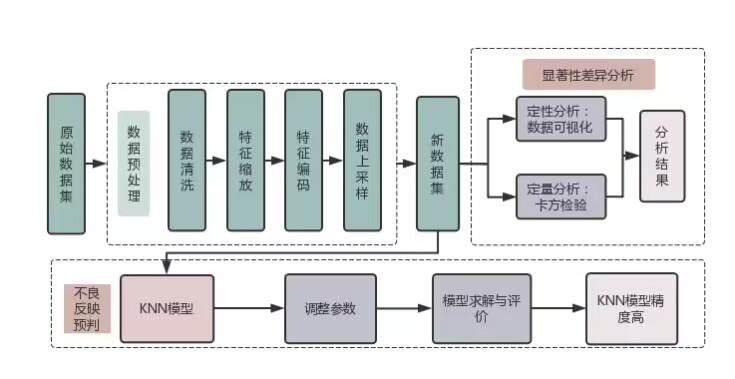
\includegraphics[width=0.95\textwidth]{流程图1.png} 
	\caption{问题一全过程流程图} 
	\label{Fig.main10001} 
\end{figure}

\subsection{第二题流程图}

\begin{figure}[H] % 这个H不要动!
	\centering % 不要动!
	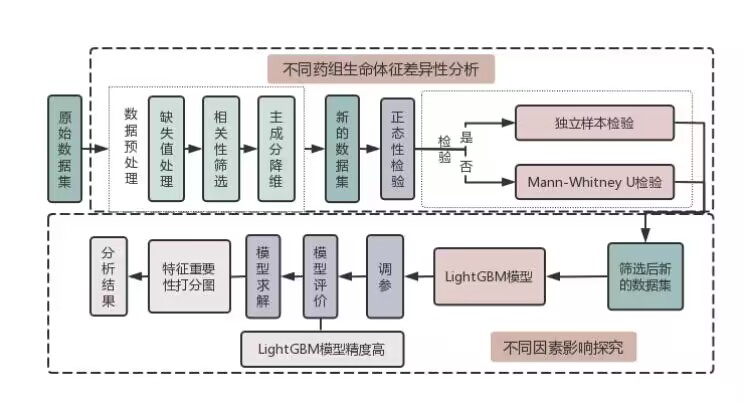
\includegraphics[width=0.95\textwidth]{流程图2.png} 
	\caption{问题二全过程流程图} 
	\label{Fig.main10002} 
\end{figure}

\subsection{第三题流程图}

\begin{figure}[H] % 这个H不要动!
	\centering % 不要动!
	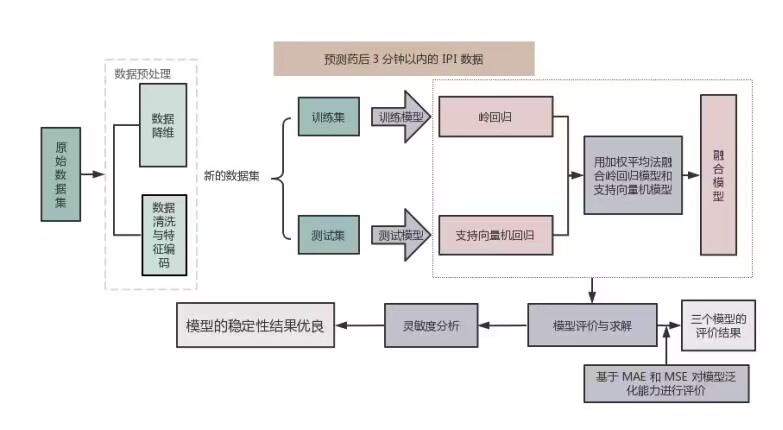
\includegraphics[width=0.95\textwidth]{流程图3.png} 
	\caption{问题三全过程流程图} 
	\label{Fig.main10003} 
\end{figure}

\subsection{第四题流程图}

\begin{figure}[H] % 这个H不要动!
	\centering % 不要动!
	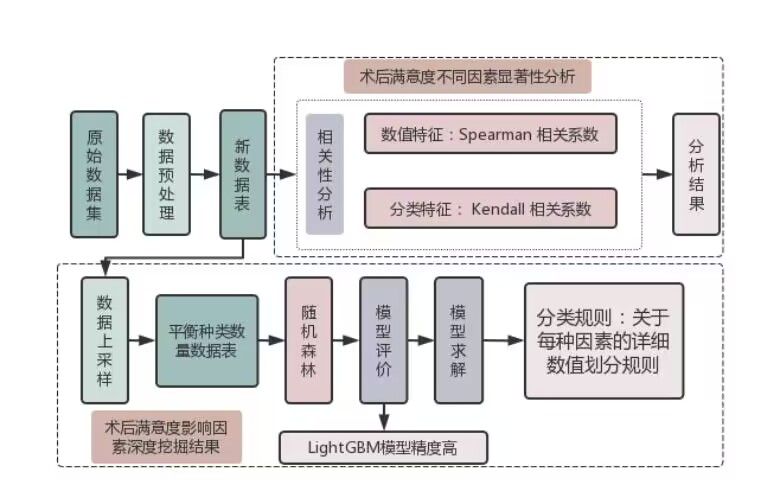
\includegraphics[width=0.95\textwidth]{流程图4.png} 
	\caption{问题四全过程流程图} 
	\label{Fig.main10004} 
\end{figure}

\section{附录:图表}

\subsection{完整KNN测试的混淆矩阵、ROC图}

\begin{figure}[H] % 这个H不要动!
	\centering % 不要动!
	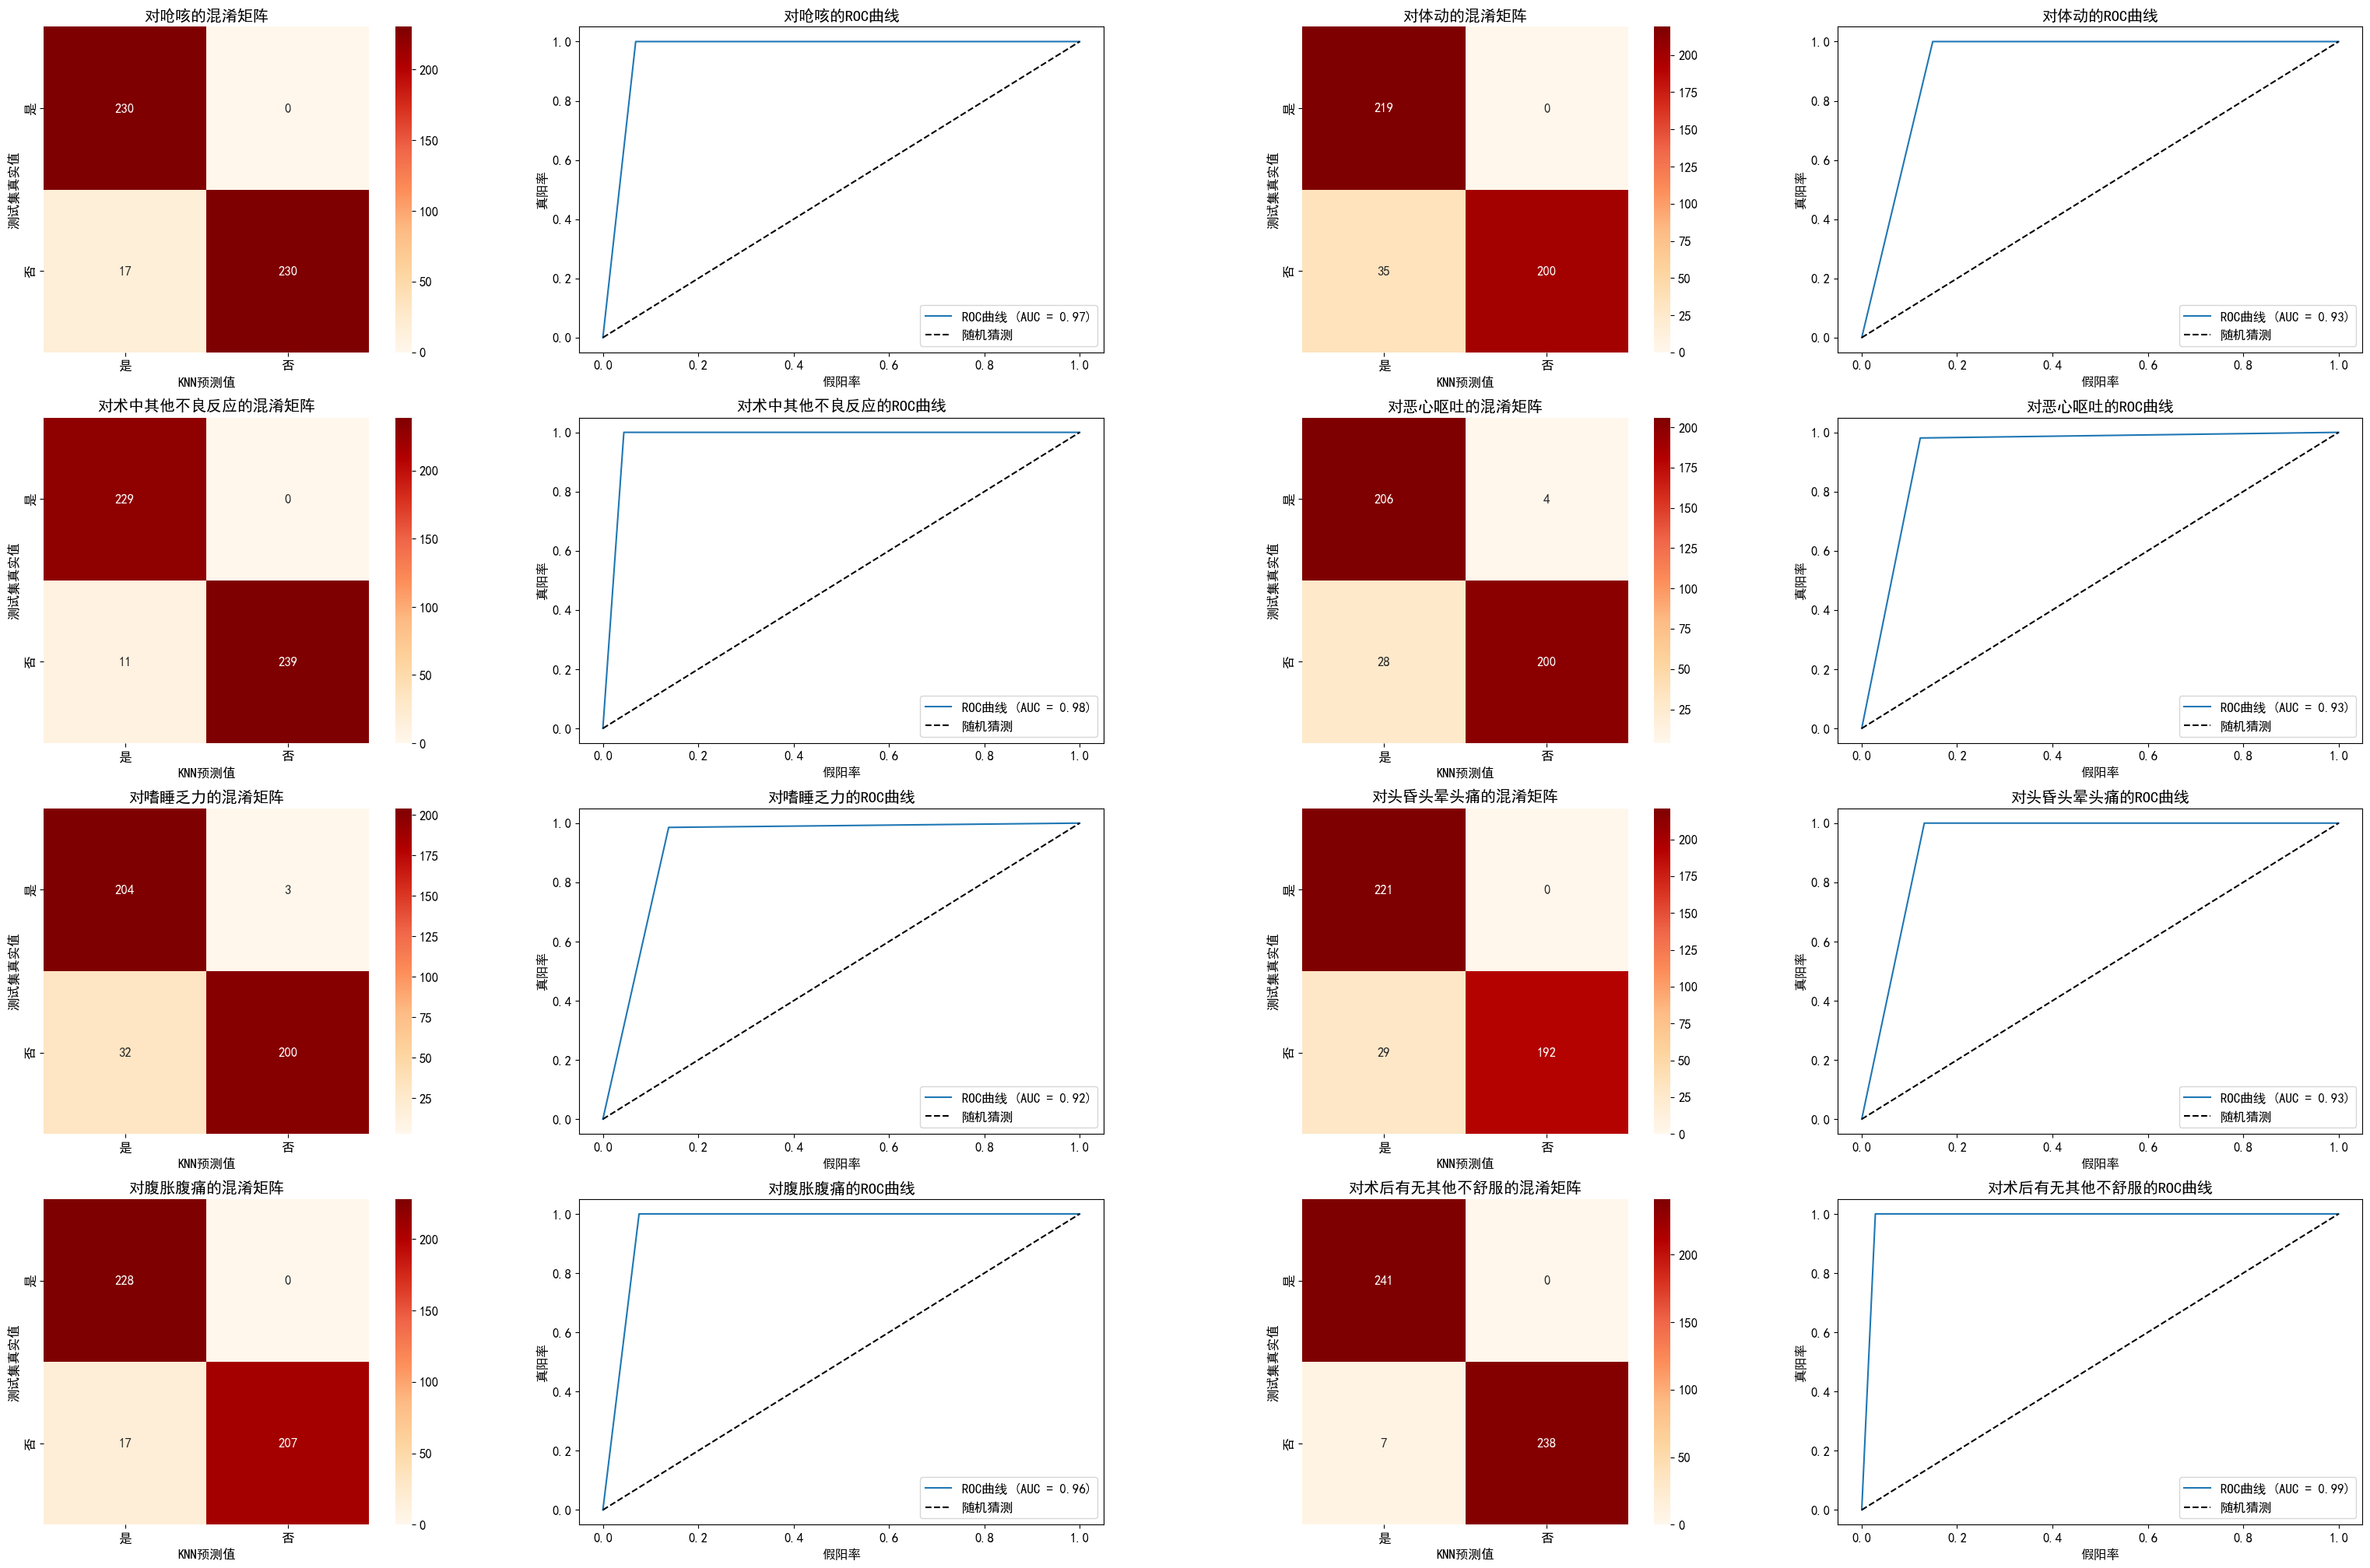
\includegraphics[width=0.95\textwidth]{附录1.png} 
	\caption{完整KNN测试结果的混淆矩阵和ROC图} 
	\label{Fig.main10005} 
\end{figure}

\subsection{六次回归的灵敏度分析图}

\begin{figure}[H] % 这个H不要动!
	\centering % 不要动!
	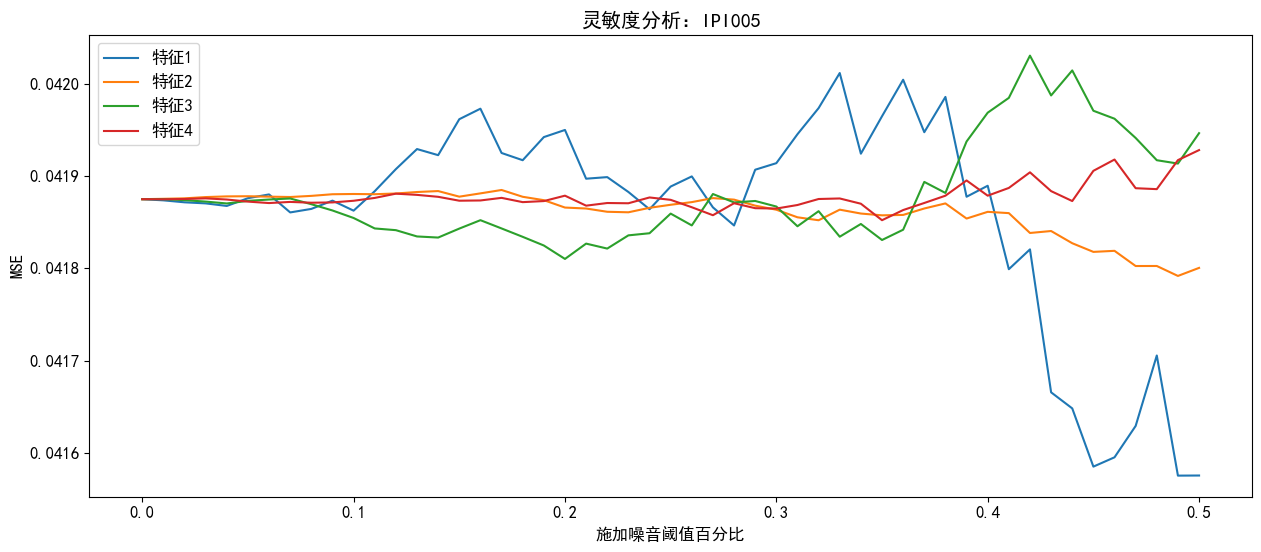
\includegraphics[width=0.95\textwidth]{附录2-1.png} 
	\label{Fig.main10016} 
\end{figure}

\begin{figure}[H] % 这个H不要动!
	\centering % 不要动!
	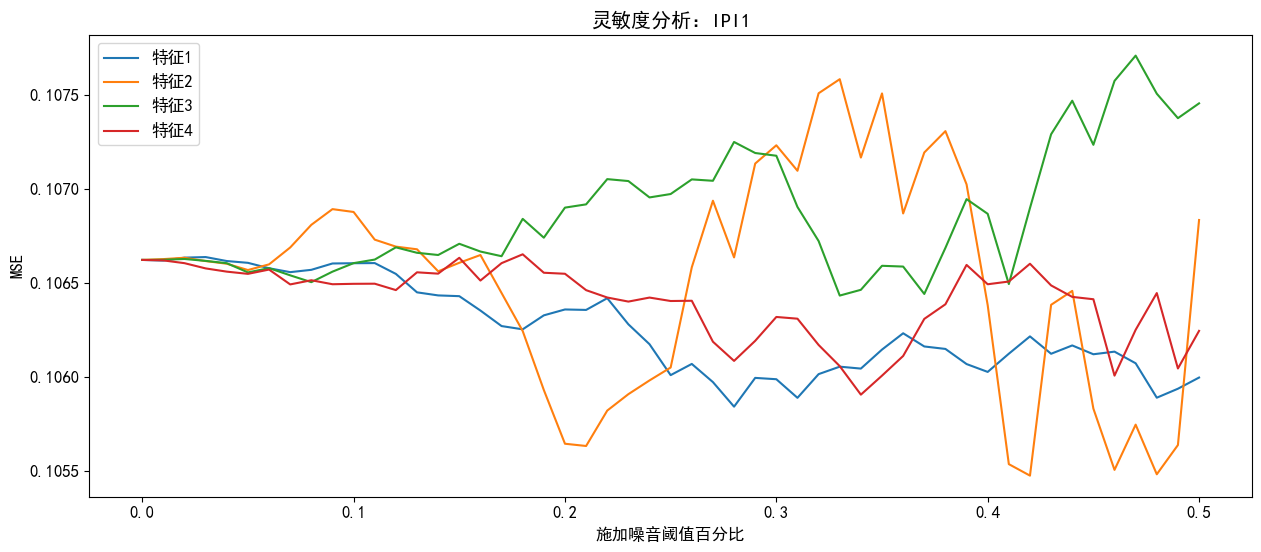
\includegraphics[width=0.95\textwidth]{附录2-2.png} 
	\label{Fig.main1002} 
\end{figure}

\begin{figure}[H] % 这个H不要动!
	\centering % 不要动!
	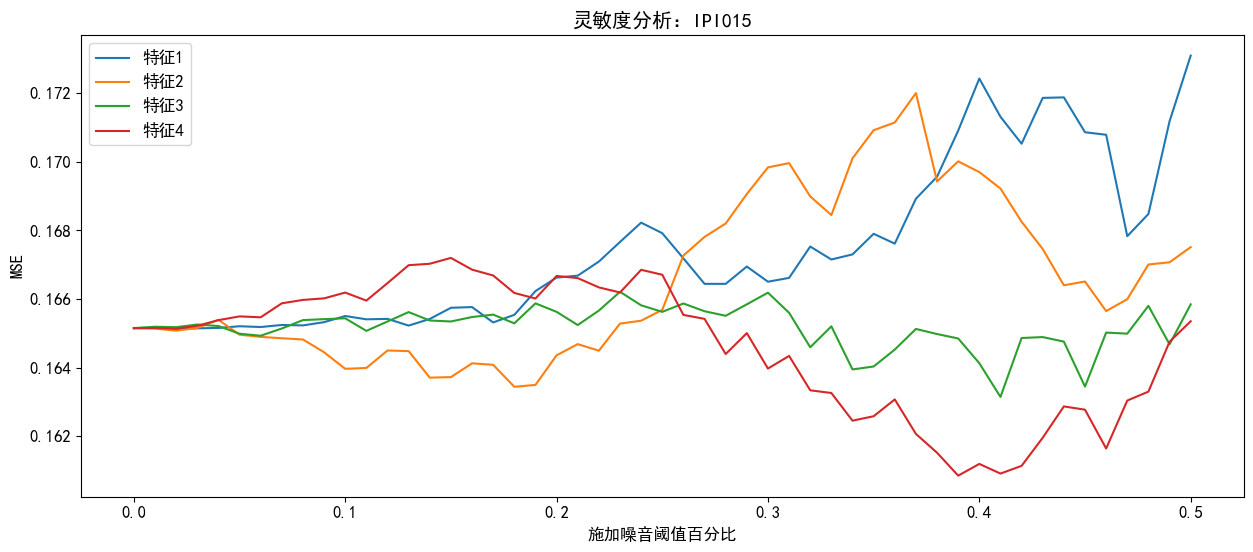
\includegraphics[width=0.95\textwidth]{附录2-3.png} 
	\label{Fig.main1003} 
\end{figure}

\begin{figure}[H] % 这个H不要动!
	\centering % 不要动!
	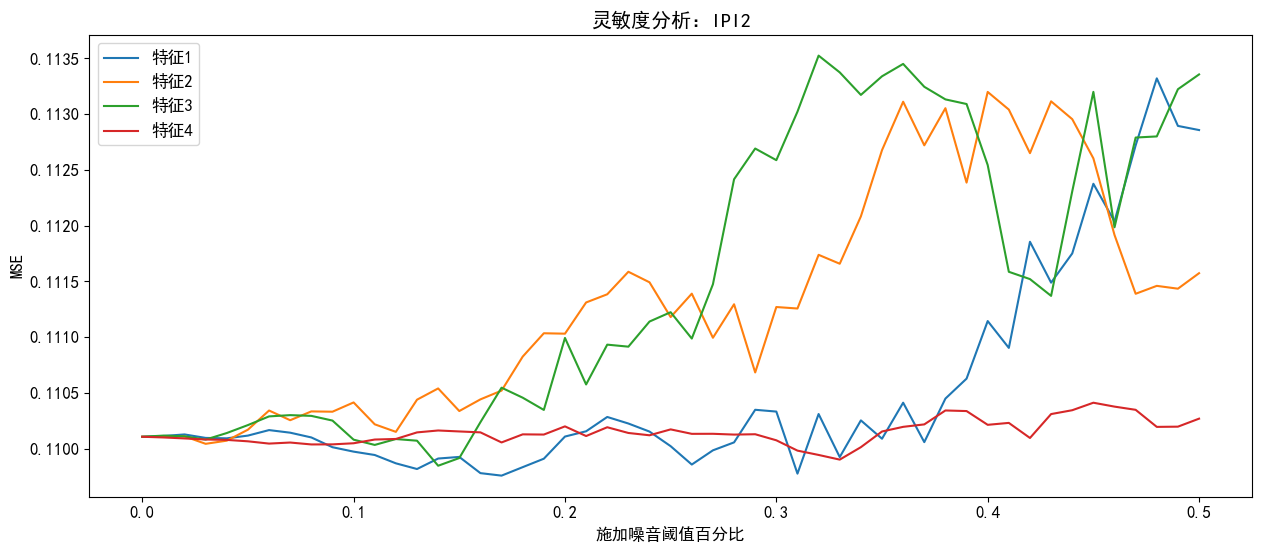
\includegraphics[width=0.95\textwidth]{附录2-4.png} 
	\label{Fig.main1004} 
\end{figure}

\begin{figure}[H] % 这个H不要动!
	\centering % 不要动!
	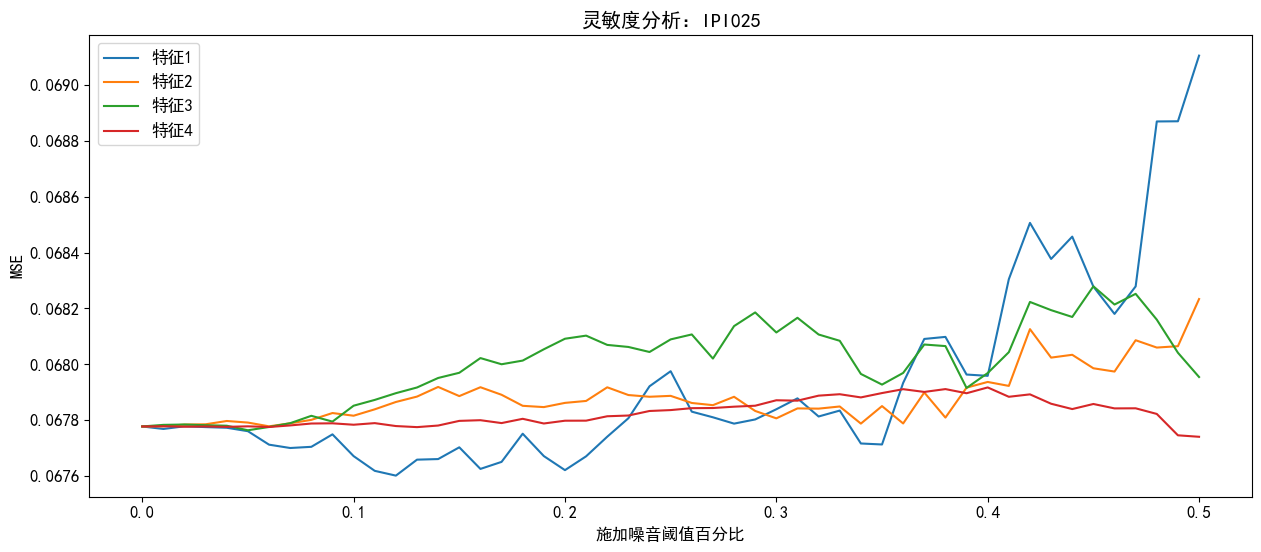
\includegraphics[width=0.95\textwidth]{附录2-5.png} 
	\label{Fig.main1005} 
\end{figure}

\begin{figure}[H] % 这个H不要动!
	\centering % 不要动!
	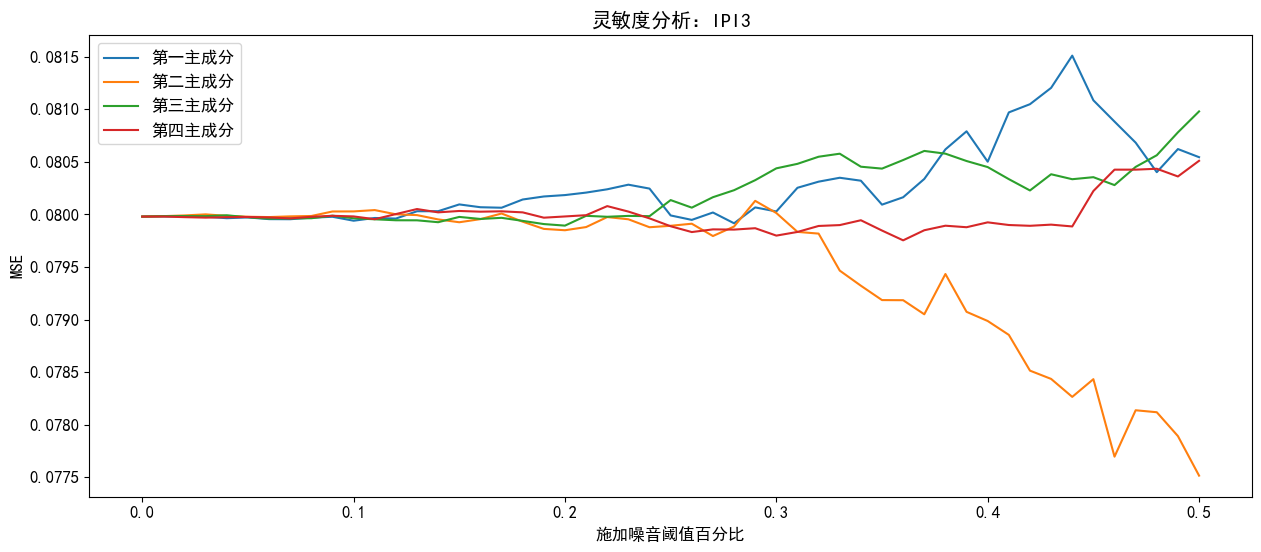
\includegraphics[width=0.95\textwidth]{附录2-6.png} 
	\label{Fig.main1006} 
\end{figure} 


\section{附录:代码}

附录代码仅为重要功能实现部分,完整代码参照提交的附件,附件内代码均为ipynb(Jupyter Notebook),路径均为相对路径,可以直接运行。

\subsection{卡方检验}

\begin{lstlisting}[language=Python]
# 创建一个交叉表格,以Sex和Category作为行列索引
cross_table = pd.crosstab(df1['镇静药名称'], df1['呛咳'])

# 进行卡方检验,并返回卡方值、p值、自由度和期望值等相关信息
chi2, p_value, dof, expected = stats.chi2_contingency(cross_table)

# 输出检验结果
# print(f"卡方值: {chi2}")
# print(f"p值: {p_value}")
# print(f"自由度: {dof}")
# print(f"期望值: \n{expected}")

if p_value < 0.05:
    print('关于呛咳,两种药有显著差异')
else:
    print('关于呛咳,两种药没有显著差异')
\end{lstlisting}

\subsection{KNN模型建立与评价}

\begin{lstlisting}[language=Python]
# ----------------------------------------------
#                     模型准备
# ----------------------------------------------
# 特征空间:独热编码
X = pd.get_dummies(df2[['性别','年龄','身高','体重','有无手术史','有无既往史',
          '是否吸烟','是否酗酒','镇静药名称']])

# 数据归一化
model = MinMaxScaler()
X[['年龄','身高','体重']] = model.fit_transform(df2[['年龄','身高','体重']])

# 字符串换成数字
df2["呛咳"] = df2["呛咳"].map({"有": 1, "无": 0})
df2["体动"] = df2["体动"].map({"有": 1, "无": 0})
df2["术中其他"] = df2["术中其他"].map({"有": 1, "无": 0})
df2["是否恶心呕吐"] = df2["是否恶心呕吐"].map({"是": 1, "否": 0})
df2["是否头晕头昏头痛"] = df2["是否头晕头昏头痛"].map({"是": 1, "否": 0})
df2["是否嗜睡乏力"] = df2["是否嗜睡乏力"].map({"是": 1, "否": 0})
df2["是否腹胀腹痛"] = df2["是否腹胀腹痛"].map({"是": 1, "否": 0})
df2["有无其他不舒服"] = df2["有无其他不舒服"].map({"是": 1, "否": 0})



# ----------------------------------------------
#                   上采样
# ----------------------------------------------
# 创建上采样对象
ros = RandomOverSampler(random_state=42)
# 对数据进行上采样
X_resampled, y_resampled = ros.fit_resample(X, df2.呛咳)

# 定义参数搜索空间
param_grid = {
    'n_neighbors': np.arange(1, 11),
    'weights': ['uniform', 'distance'],
    'algorithm': ['auto', 'ball_tree', 'kd_tree', 'brute'],
    'leaf_size': np.arange(10, 51, 10),
    'p': [1, 2, 3]
}

# ----------------------------------------------
#               GridSearchCV调参
# ----------------------------------------------
# 初始化KNN模型
knn = KNeighborsClassifier()

# 使用网格搜索进行调参
grid_search = GridSearchCV(knn, param_grid=param_grid, cv=5)
grid_search.fit(X_resampled, y_resampled)

# 输出最佳参数和最佳得分
print("Best parameters: {}".format(grid_search.best_params_))
print("Best cross-validation score: {:.2f}".format(grid_search.best_score_))

# ----------------------------------------------
#           以“呛咳”为例的KNN预测实现
# ----------------------------------------------
# 创建上采样对象
ros = RandomOverSampler(random_state=42)
# 对数据进行上采样
X_resampled, y_resampled = ros.fit_resample(X, df2.呛咳)

# 划分数据集
X1_train, X1_test, y1_train, y1_test = train_test_split(X_resampled, y_resampled, test_size=0.2, random_state=0)

Model = KNeighborsClassifier(algorithm='auto', leaf_size=10, 
                            n_neighbors=1, p=3, weights='uniform')
y1_pred = Model.fit(X1_train, y1_train).predict(X1_test)

# 模型评价
print("评估数据结果打印:\n", classification_report(y1_test, y1_pred))

# ----------------------------------------------
#             混淆矩阵与ROC曲线
# ----------------------------------------------
mat1 = confusion_matrix(y1_test, y1_pred, 
                labels=[1, 0])
fpr1, tpr1, thresholds1 = roc_curve(y1_test, y1_pred)
auc1 = roc_auc_score(y1_test, y1_pred)

plt.subplot(1, 2, 1)
sns.heatmap(mat1, annot=True, square="equal", cmap="OrRd", fmt="d",
    xticklabels=["是", "否"], 
    yticklabels=["是", "否"])
plt.xlabel("KNN预测值")
plt.ylabel("测试集真实值")
plt.title("对呛咳的混淆矩阵")

plt.subplot(1, 2, 2)
# 绘制ROC曲线和y=x的对角线
plt.plot(fpr1, tpr1, label='ROC曲线 (AUC = {:.2f})'.format(auc1))
plt.plot([0, 1], [0, 1], 'k--', label='随机猜测')
plt.xlabel('假阳率')
plt.ylabel('真阳率')
plt.title('对呛咳的ROC曲线')
plt.legend()
\end{lstlisting}


\subsection{主成分分析法}

\begin{lstlisting}[language=Python]
# ----------------------------------------------
#   先试探,用可视化图确定具体降维多少
# ----------------------------------------------
# 创建PCA对象并进行降维
pca = PCA(n_components=49)
df_try = pca.fit_transform(df3[['sbp00', 'dbp00', 'petco200', 'RR00', 'spo200', 'HR00', 'IPI00', 'moaas00',
    'petco2005','RR005','spo2005','HR005','IPI005','moaas005','sbp1','dbp1',
    'petco21','RR1','spo21','HR1','IPI1','moaas1','sbpjinjing','dbpjinjing','petco2jinjing',
    'RRjinjing','spo2jinjing','HRjinjing','IPIjinjing','moaasjinjing','petco2015',
    'RR015','spo2015','HR015','IPI015','moaas015','sbp2','dbp2','petco22','RR2','spo22',
    'HR2','IPI2','moaas2','petco2025','RR025','spo2025','HR025','IPI025',
    'moaas025','sbp3','dbp3','petco23','RR3','spo23','HR3','IPI3','moaas3','sbp5',
    'dbp5','petco25','RR5','spo25','HR5','IPI5','moaas5','sbp7','dbp7','petco27',
    'RR7','spo27','HR7','IPI7','moaas7','sbpjieshu',
    'dbpjieshu','petco2jieshu','RRjieshu','spo2jieshu','HRjieshu','IPIjieshu']])

# 绘制主成分方差解释比例图
plt.figure(figsize=(20, 5))
plt.plot(np.cumsum(pca.explained_variance_ratio_))
plt.xlabel('降维所得个数')
plt.ylabel('主成分的方差解释比例')
plt.title('主成分的方差解释比例图')
plt.show()

# ----------------------------------------------
#   主成分分析法实现数据降维
# ----------------------------------------------
# 创建PCA对象并进行降维
pca = PCA(n_components=10)
df4 = pd.DataFrame(pca.fit_transform(df3.drop(['镇静药名称','性别','年龄','身高',
                                            '体重','有无手术史','有无既往史','是否吸烟',
                                            '是否酗酒','有无PONV','有无晕动史'], axis=1)))
\end{lstlisting}


\subsection{独立样本检验}

\begin{lstlisting}[language=Python]
# ----------------------------------------------
#             进行正态性检验
# ----------------------------------------------
stat, p = normaltest(df[1])
if p < 0.05:
    print('参数检验')
else:
    print('非参数检验')
    
# ----------------------------------------------
#                   独立样本t检验
# ----------------------------------------------
# 将标签数据根据性别分成两组
e1 = df.loc[df['镇静药组'] == 1, 'label1']
e2 = df.loc[df['镇静药组'] == 0, 'label1']

# 进行独立样本t检验
fvalue, pvalue = ttest_ind(e1, e2)

# 输出结果
print("F值为:", fvalue)
print("p值为:", pvalue)

# ----------------------------------------------
#               Mann-Whitney U
# ----------------------------------------------
# 将标签数据根据性别分成两组
e1 = df.loc[df['镇静药组'] == 1, 'label2']
e2 = df.loc[df['镇静药组'] == 0, 'label2']

# 进行Mann-Whitney U检验
fvalue, pvalue = mannwhitneyu(e1, e2)

# 输出结果
print("F值为:", fvalue)
print("p值为:", pvalue)

\end{lstlisting}

\subsection{LightGBM建模与特征重要性分析}

\begin{lstlisting}[language=Python]
# ----------------------------------------------
#               划分数据集
# ----------------------------------------------
X1_train, X1_test, y1_train, y1_test = train_test_split(X, df[3], train_size=0.8, random_state=1)


# ----------------------------------------------
#              GridSearchCV调参
# ----------------------------------------------
model = lgb.LGBMRegressor(learning_rate=0.1)
param = {
        "max_depth":[4, 7, 10],
        "num_leaves":[300, 600, 900],
        "n_estimators":[10, 70, 130],
        'min_child_samples': [18, 20, 22],
        'min_child_weight':[0.001, 0.002]
        }

grid_search3 = GridSearchCV(model, n_jobs=-1, param_grid=param, cv=5, scoring="neg_mean_squared_error")
grid_search3.fit(X1_train, y1_train)
grid_search3.best_estimator_, grid_search3.best_score_

X1_train, X1_test, y1_train, y1_test = train_test_split(X, df[3], train_size=0.8, random_state=1)


# ----------------------------------------------
#            LightGBM模型建立
# ----------------------------------------------
model1 = lgb.LGBMRegressor(max_depth=7, min_child_samples=22, n_estimators=10,num_leaves=300)
y1_pred = model1.fit(X1_train, y1_train).predict(X1_test)


# ----------------------------------------------
#            LightGBM模型评价
# ----------------------------------------------
# Mean Absolute Error(平均绝对误差)
print(mean_absolute_error(y1_test, y1_pred))

# Mean Squared Error(均方误差)
print(mean_squared_error(y1_test, y1_pred))

names = ['镇静药名称','性别','年龄','身高','体重','有无手术史','有无既往史',  
        '是否吸烟','是否酗酒','有无PONV','有无晕动史']

# ----------------------------------------------
#            LightGBM特征重要性打分
# ----------------------------------------------
plt.figure(figsize=(15, 5))
plt.title("生命体征第三主成分的影响探究")
plt.xlabel("可能的影响因素")
plt.ylabel("特征重要性打分")
plt.bar(names, model1.feature_importances_, color='b')
plt.show()
\end{lstlisting}

\subsection{回归器的模型融合与灵敏度分析}

\begin{lstlisting}[language=Python]
# ----------------------------------------------
#            岭回归的实现
# ----------------------------------------------
# 模型初始化
ridge = Ridge(alpha=1)
# 模型训练、模型预测
y1_pred1 = ridge.fit(X1_train, y1_train).predict(X1_test)
# Mean Squared Error(均方误差)
MSE_1 = mean_squared_error(y1_test, y1_pred1)
# Mean Absolute Error(平均绝对误差)
MAE_1 = mean_absolute_error(y1_test, y1_pred1)

print(MSE_1)
print(MAE_1)

# ----------------------------------------------
#            支持向量机的实现
# ----------------------------------------------
# 支持向量机
svr = SVR(kernel='rbf')
# 模型训练、模型预测
y1_pred2 = svr.fit(X1_train, y1_train).predict(X1_test)
# Mean Squared Error(均方误差)
MSE_2 = mean_squared_error(y1_test, y1_pred2)
# Mean Absolute Error(平均绝对误差)
MAE_2 = mean_absolute_error(y1_test, y1_pred2)

print(MSE_2)
print(MAE_2)

# ----------------------------------------------
#            加权平均法的实现
# ----------------------------------------------
w1 = 1 / MSE_1
w2 = 1 / MSE_2
w1_normalized = w1 / (w1 + w2)
w2_normalized = w2 / (w1 + w2)

y1_pred = w1_normalized * y1_pred1 + w2_normalized * y1_pred2

print(mean_squared_error(y1_test, y1_pred))
print(mean_absolute_error(y1_test, y1_pred))


# ----------------------------------------------
#            灵敏度分析
# ----------------------------------------------
def analysis(X1_test):
    # 接受过噪音的X_test得分情况
    score_1, score_2, score_3, score_4 = [], [], [], []

    for j in range(0, 4):

        # 备份新的X_test用于噪音处理
        df1 = np.array(X1_test.copy())
        # 打印X_test的维数,方便后面做循环
        m, n = np.array(X1_test).shape
        # 噪音
        error = np.ones(shape=(m, 1))

        # 按0到0.5的比例对X_test进行噪音处理
        for i in np.linspace(0, 0.5, 51):

            # 施加对应比例噪音并添加到X_test上,产生新的测试集特征df2
            error[:, 0] = np.random.uniform(-i * df1[:, j], i * df1[:, j])
            df1[:, j] = df1[:, j] + error[:, 0]
            df2 = pd.DataFrame(df1)
            df2.columns = ['特征1', '特征2', '特征3', '特征4']

            # 构建完数据后预测、打分
            y_pred1 = pd.DataFrame(ridge.predict(df2))
            y_pred2 = pd.DataFrame(svr.predict(df2))
            MSE_1 = mean_squared_error(y1_test, y_pred1)
            MSE_2 = mean_squared_error(y1_test, y_pred2)

            w1 = 1 / MSE_1
            w2 = 1 / MSE_2
            w1_normalized = w1 / (w1 + w2)
            w2_normalized = w2 / (w1 + w2)

            y_pred = w1_normalized * y_pred1 + w2_normalized * y_pred2
        
            if j == 0:
                score_1.append(mean_squared_error(y1_test, y_pred))
            elif j == 1:
                score_2.append(mean_squared_error(y1_test, y_pred))
            elif j == 2:
                score_3.append(mean_squared_error(y1_test, y_pred))
            else:
                score_4.append(mean_squared_error(y1_test, y_pred))
    
    return score_1, score_2, score_3, score_4

score_1, score_2, score_3, score_4 = analysis(X1_test)

plt.figure(figsize=(15, 6))
plt.rcParams["font.sans-serif"] = ["SimHei"]
plt.rcParams['font.size'] = 12  # 字体大小
plt.rcParams['axes.unicode_minus'] = False  # 正常显示负号
plt.xlabel("施加噪音阈值百分比")
plt.ylabel("MSE")

plt.plot(np.linspace(0, 0.5, 51), score_1, label="特征1")
plt.plot(np.linspace(0, 0.5, 51), score_2, label="特征2")
plt.plot(np.linspace(0, 0.5, 51), score_3, label="特征3")
plt.plot(np.linspace(0, 0.5, 51), score_4, label="特征4")

plt.title("灵敏度分析:IPI005")
plt.legend()
plt.show()
\end{lstlisting}



\subsection{随机森林的建模与树状图导出}


\begin{lstlisting}[language=Python]
# ----------------------------------------------
#            模型准备
# ----------------------------------------------
X = df1.drop("rating", axis=1)
y = df1.rating


# ----------------------------------------------
#            上采样
# ----------------------------------------------
# 创建上采样对象
ros = RandomOverSampler(random_state=42)
# 对数据进行上采样
X_resampled, y_resampled = ros.fit_resample(X, y)

X_train, X_test, y_train, y_test = train_test_split(X_resampled, y_resampled, test_size=0.2, random_state=0)


# ----------------------------------------------
#            随机森林建模与评价
# ----------------------------------------------
Model = RandomForestClassifier(max_depth=3, n_estimators=1000)
y_pred = Model.fit(X_train, y_train).predict(X_test)

# 打印分类模型最好的评价系统
print("评估数据结果打印:\n", classification_report(y_test, y_pred))

# ----------------------------------------------
#            树状图导出
# ----------------------------------------------
plt.figure(figsize=(20, 10))
estimator = Model.estimators_[5]
estimator.fit(X_train, y_train)
plot_tree(estimator, filled=True, max_depth=3, feature_names=X.columns)

plt.title("随机森林分类树状图")
plt.show()
\end{lstlisting}

